% kapitel4.tex
\chapter{Wagner Struktur}
\label{cha:wagnerstruktur}

In diesem Kapitel soll Theorem \ref{eq:Theorem36} genauer betrachtet werden.
Zunächst werden einige Baumstrukturen eingeführt, die den $3$-Zusammenhang herstellen können.
Anschließend werden \dd-Separatoren behandelt und eine Formulierung von dem Theorem von Wagner, das in Theorem \ref{eq:Theorem36} benutzt wurde, vorgestellt.
Letztlich werden die gewonnen Erkenntnisse zu einer neuen Struktur zusammengefasst, die als Zertifikat für den Algorithmus von Kezdy und McGuinness dienen kann und dieser entsprechend angepasst.

\subsection{$2$-Zusammenhang}

\begin{wrapfigure}{r}{6cm}
  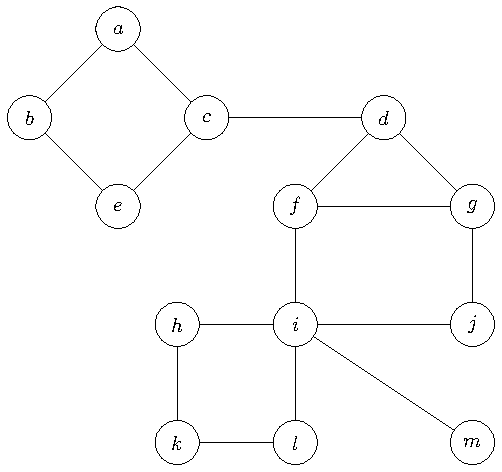
\includegraphics[width=6cm]{bilder/1-Block-Tree1.pdf}
  \caption{Ein nicht $2$-zusammenhängender Graph $G_1$.}
  \label{fig:1-Block-Tree1}
\end{wrapfigure}
\begin{definition}
  Als \emph{Block} eines Graphen $G$ wird jeder seiner maximalen Teilgraphen bezeichnet, der keinen $1$-Separator enthält -- als $2$-zusammenhängend ist.
  Je zwei Blöcke haben maximal einen gemeinsamen Knoten, der einen $1$-Separator in $G$ bildet.
  Der \emph{Block-Cut Tree} von $G$ ist ein Baum, der für jeden Block von $G$ einen Knoten besitzt und für jeden Separator eine Kante\cite{BoM08}.
\end{definition}
Als Beispiel wird in \Abb \ref{fig:1-Block-Tree1} ein Graph mit dazugehörigem Block-Cut Tree in \Abb \ref{fig:1-Block-Tree2} gezeigt.
Die Knoten des Block-Cut Tree sind als durchgezogene Linien angegeben, in jedem dieser Knoten findet sich ein $2$-zusammenhängender Teilgraph aus $G_1$. %TODO: Laufzeit
\begin{figure}[H]
  \centering
  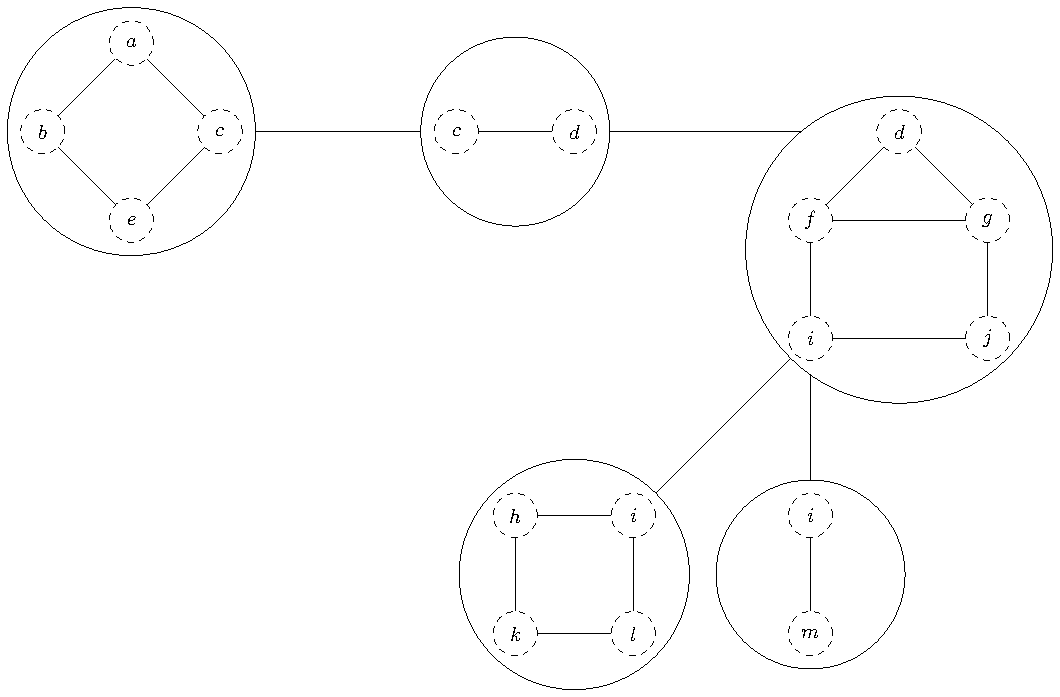
\includegraphics[width=\textwidth,height=\textheight,keepaspectratio]{bilder/1-Block-Tree2.pdf}
  \caption{Der Block-Cut Tree zu $G$ aus \Abb \ref{fig:1-Block-Tree1}.}
  \label{fig:1-Block-Tree2}
\end{figure}

In \cite{Li11} stellt Li eine Erweiterung zum Block-Cut Tree vor, die als \emph{$1$-Block-Tree} bezeichnet wird, da neben den Blöcken auch $1$-Separatoren enthalten sind.

\begin{definition}
  Seien für einen Graphen $G$ die Knoten seines Block-Cut Trees $T_{bc} = (V_{T_{bc}}, E_{T_{bc}})$ als Blockknoten bezeichnet.
  Der \emph{$1$-Block-Tree} von $G$ ist ein Baum $T_{(1)} = (V_{(1)}, E_{(1)})$.
  Dann gilt $V_{(1)} \subseteq V_{T_{bc}}$.
  Außerdem enthält $T_{(1)}$ einen zusätzlichen Knoten $c$ für jede Kante $(u, v) \in E_{T_{bc}}$, sodass $\{(u, c), (c, v)\} \subseteq E_{(1)}$ und $E_{T_{bc}} \cap E_{(1)} = \emptyset$ gilt.
  Dabei wird $c$ als Cliquenknoten bezeichnet und beinhaltet genau den $1$-Separator, den die zu $u$ und $v$ gehörenden Teilgraphen in $G$ als gemeinsamen Knoten besitzen.
\end{definition}

Ein Beispiel findet sich in \Abb \ref{fig:1-Block-Tree3}.
Es kann beobachtet werden, dass die in Blockknoten enthaltenen Teilgraphen identisch zu den augmentierten Komponenten sind, die im Algorithmus von Kezdy und McGuinness in Schritt \ref{item:algorithmus11} durch $1$-Separatoren gebildet werden.
\begin{figure}[H]
  \centering
  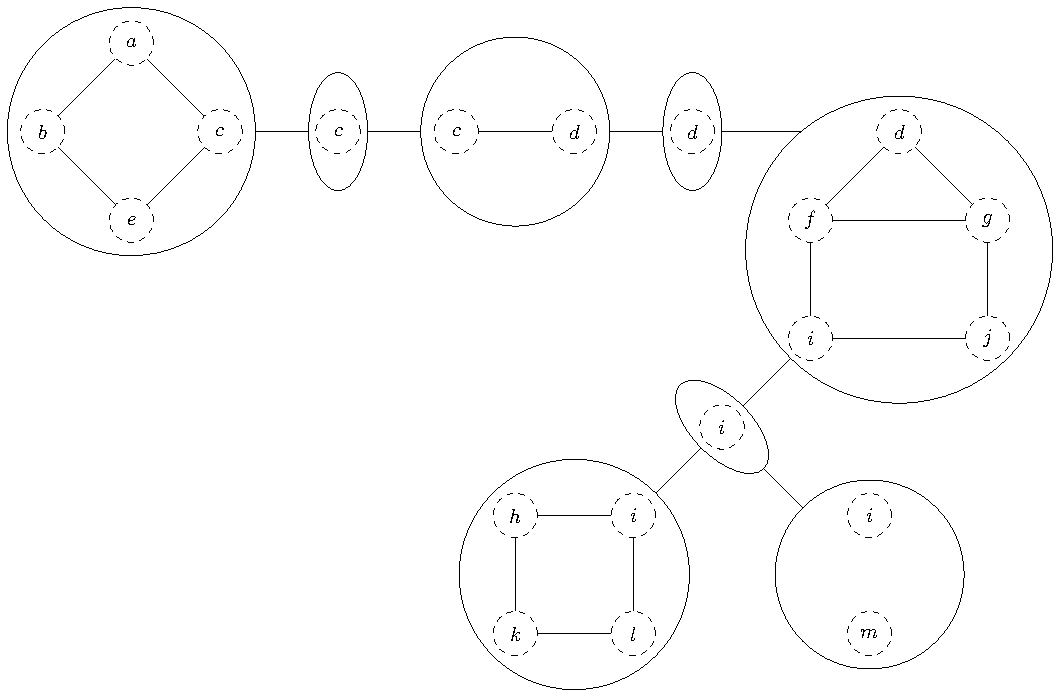
\includegraphics[width=\textwidth,height=\textheight,keepaspectratio]{bilder/1-Block-Tree3.pdf}
  \caption{Der $1$-Block-Tree zu $G$ aus \Abb \ref{fig:1-Block-Tree2}.
           Die Cliquenknoten sind ovalförmig dargestellt.}
  \label{fig:1-Block-Tree3}
\end{figure}


\subsection{$3$-Zusammenhang}

Nachdem durch Block-Cut Trees \bzw $1$-Block-Trees der $2$-Zusammenhang in allen Blockknoten hergestellt wurde, können die darin enthaltenen Teilgraphen jeweils als Eingabe für einen SPQR-Baum genutzt werden, um $3$-zusammenhängende Komponenten zu erzeugen.
Die folgende Definition dazu ist \cite{GuM00} entnommen.

\begin{figure}[H]
  \centering
  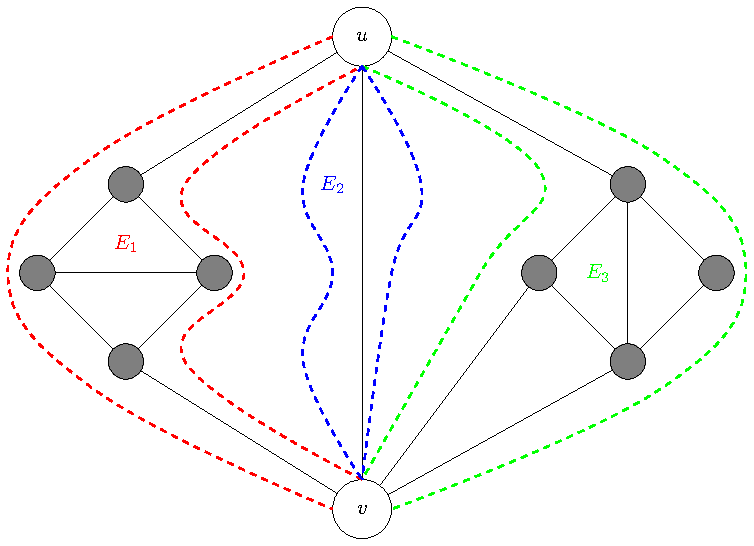
\includegraphics[width=\textwidth,height=\textheight,keepaspectratio]{bilder/Split-Kantenmengen.pdf}
  \caption{Unterteilung der Kanten in drei Mengen $E_1$, $E_2$ und $E_3$ anhand des Knotenpaares $\{u, v\}$.}
  \label{fig:Split-Kantenmengen}
\end{figure}

\begin{definition}
  Sei $G = (V, E)$ ein $2$-zusammenhängender Graph.
  Als \emph{Split Pair} $\{u, v\}$ wird entweder ein adjazentes Knotenpaar oder ein $2$-Separator bezeichnet, ein \emph{maximales Split Pair} $\{s, t\}$ für $\{u, v\}$ teilt den Graphen so auf, dass $u$, $v$, $s$, und $t$ in einer $3$-zusammenhängenden Komponente liegen.
  Eine \emph{Split Component} für ein Split Pair ist entweder eine Kante zwischen diesem oder der maximale Teilgraph, für den es kein Split Pair mehr ist.
  Ein solches Knotenpaar teilt die Kanten in die Mengen $E_1, ..., E_k$, sodass eine Menge $E_i$ alle Pfade enthält, die $u$ oder $v$ höchstens als Endpunkte haben.
  Dabei enthält $E_i$ entweder einen Teilgraphen von $G$, der nur das Knotenpaar enthält, oder einen für den das Knotenpaar kein $2$-Separator ist.
  \footnote {In \Abb \ref{fig:Split-Kantenmengen} ist ein $2$-zusammenhängender Graph skizziert, in dem $\{u, v\}$ eingezeichnet ist, sowie farblich hervorgehoben die dadurch entstehende Unterteilung in Kantenmengen.}
  Der SPQR-Baum $T_{SPQR}$ von $G$ ist ein Baum, der $G$ anhand jedem Split Pair $\{u, v\}$ rekursiv aufteilt und die entstehenden Minoren mit \emph{S}, \emph{P}, \emph{Q} oder \emph{R} markiert:
  \begin{itemize}
    \item \textbf{Q}: Tritt der Randfall auf, dass $G$ nur eine einzige Kante $(u, v)$ besitzt, dann enthält der SPQR-Baum einen einzelnen Q-Knoten, der auf $G$ verweist.
    \item \textbf{P}: Entstehen durch das Knotenpaar die Kantenmengen $E_1, ..., E_k$ mit $k \geq 3$, dann wird ein P-Knoten hinzugefügt, der das Knotenpaar enthält sowie $k$ viele parallele Kanten zwischen diesem.
    \item \textbf{S}: Andernfalls teilen $u$ und $v$ die Kanten in zwei Mengen, sodass es eine Kante $(u, v) \in E$ und einen weitere Pfad gibt, der das Knotenpaar verbindet, dann enthält der hinzugefügte S-Knoten die Kante und den Pfad.
    \item \textbf{R}: Tritt keiner der obigen Fälle ein, dann seien $\{s_1, t_1\}, ..., \{s_k, t_k\}$ für $k \geq 1$ die maximalen Split Pairs für ${u, v}$ und $G_i$ für alle $1 \leq i \leq k$ die Vereinigung aller Split Components für $\{u, v\}$ außer der, die die Kante $(u, v)$ enthält.
                      Der neue R-Knoten enthält $G$, wobei jeder Teilgraph $G_i$ durch die Kante $(s_i, t_i)$ ersetzt wird.
  \end{itemize}
\end{definition}

\begin{figure}[H]
  \centering
  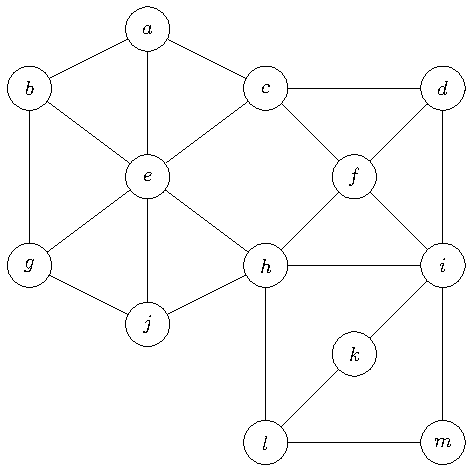
\includegraphics[width=8cm]{bilder/2-Block-Tree1.pdf}
  \caption{Ein $2$-zusammenhängender Graph $G_2$.}
  \label{fig:2-Block-Tree1}
\end{figure}

\begin{figure}[H]
  \centering
  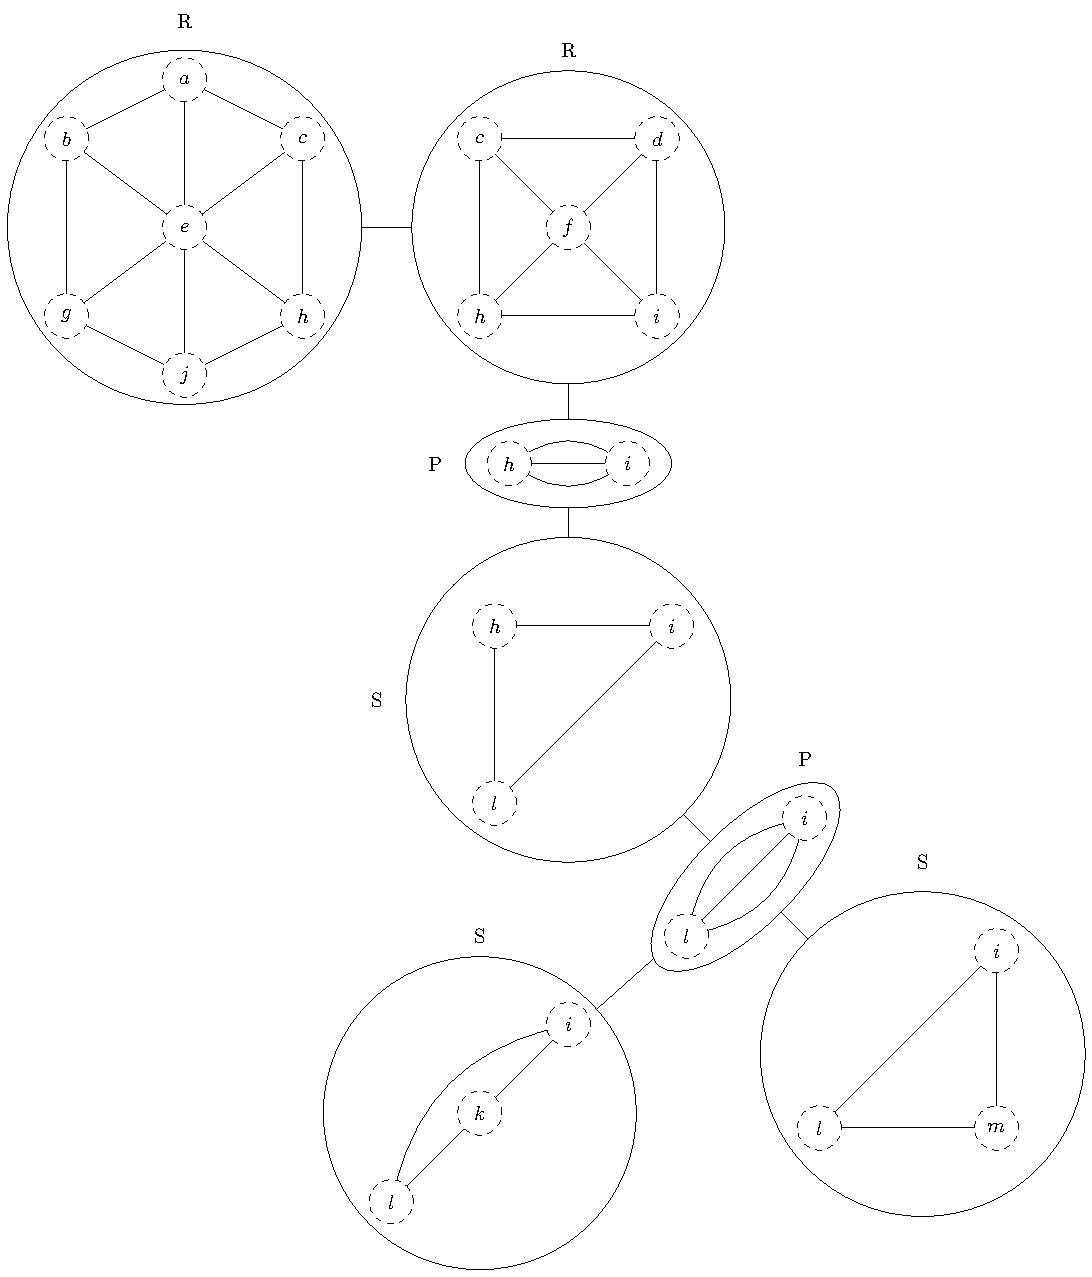
\includegraphics[width=\textwidth,height=\textheight,keepaspectratio]{bilder/SPQR-Tree.pdf}
  \caption{SPQR Baum zum Graphen $G_2$ aus \Abb \ref{fig:2-Block-Tree1}.}
  \label{fig:SPQR-Tree}
\end{figure}

Zu dem Graphen in \Abb \ref{fig:2-Block-Tree1} ist in \Abb \ref{fig:SPQR-Tree} der zugehörige SPQR Baum skizziert.
Besonders interessant sind die R-Knoten, die $3$-zusammenhängende Minoren von $G_2$ sind.
Zwar gilt das auch für die drei S-Knoten, allerdings sind Kreise generell nicht $3$-zusammenhängend, aber immer planar.

In \cite{Li11} stellt Li analog zum $1$-Block-Tree den $2$-Block-Tree vor, der aus $3$-zusammenhängende Komponenten (Blockknoten) und $2$-Separatoren (Cliquenknoten) besteht.

\begin{definition}
  Sei $G = (V_G, E_G)$ ein $2$-zusammenhängender, \kf-Minor freier Graph, dann ist der \emph{$2$-Block-Tree} $T_{(2)} = (V_{(2)}, E_{(2)})$ von $G$ wie folgt definiert.
  Bilden die Knoten $\{u, v\} \subseteq V_G$ einen $(2, j)$-Separator in $G$ für $j \geq 2$, dann seien $Z_1, ..., Z_j$ die Zusammenhangskomponenten von $G - \{u, v\}$.
  Analog zum $1$-Block-Tree wird ein Cliquenknoten für den Separator angelegt, der alle Blockknoten bestehend aus $Z_i \cup \{u, v\}$ als Nachbarn besitzt.
  Außerdem wird die Kante $(u, v)$ sowohl in den Block- als auch in dem Cliquenknoten hinzugefügt, falls sie nicht vorhanden ist.
  Ist $G$ $3$-zusammenhängend, besitzt $T_{(2)}$ einen einzelnen Blockknoten, der $G$ vollständig enthält.
\end{definition}

Ein $2$-Block-Tree zu $G_2$ aus \Abb \ref{fig:2-Block-Tree1} ist in \Abb \ref{fig:2-Block-Tree2} zu sehen.
Es ist zu beobachten, dass Knoten wie etwa $h$ oder $i$ Teil mehrerer Separatoren sein können und somit nicht nur in mehreren Graph-, sondern auch in mehreren Cliquenknoten enthalten sind.
Allerdings sind keine zwei Knoten im $2$-Block-Tree identisch.
\begin{figure}[H]
  \centering
  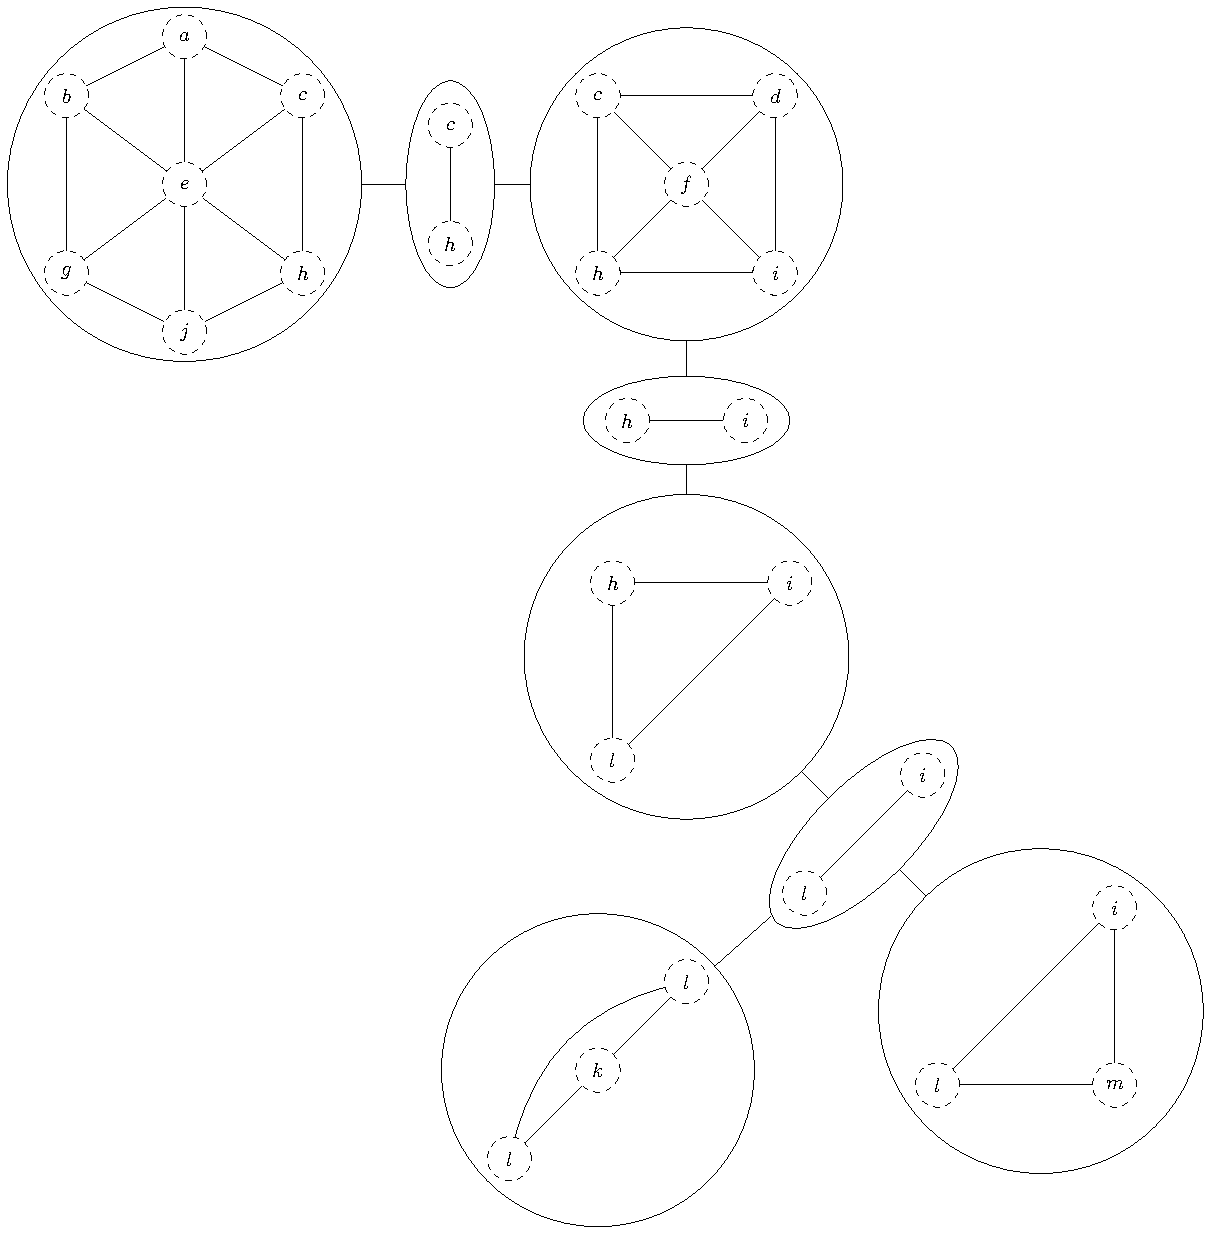
\includegraphics[width=\textwidth,height=\textheight,keepaspectratio]{bilder/2-Block-Tree2.pdf}
  \caption{$2$-Block-Tree zum Graphen aus \Abb \ref{fig:2-Block-Tree1}.
           Die Cliquenknoten sind ovalförmig dargestellt und enthalten immer genau zwei Knoten, alle übrigen sind Blockknoten.}
  \label{fig:2-Block-Tree2}
\end{figure}


\subsection{\dd-Separatoren}

\begin{definition}
  Sei $G = (V_G, E_G)$ ein $3$-zusammenhängender, \kf-Minor freier Graph, dann ist der \emph{\dd-Block-Tree} $T_{(3, 3)} = (V_{(3, 3)}, E_{(3, 3)})$ von $G$ wie folgt definiert.
  Enthält $G$ keinen $(3, j)$-Separator für $j \geq 3$, so besitzt $T_{(3, 3)}$ einen einzigen Blockknoten, der $G$ komplett enthält.
  Sei andernfalls $C$ ein Graph, der die drei Knoten eines solchen $(3, j)$-Separators als Clique beinhaltet.
  Dann werden Blockknoten in $T_{(3, 3)}$ für alle $Z_i \cup C$ mit $1 \leq i \leq j$ angelegt, wobei $Z_i$ die durch den Separator entstandenen Zusammenhangskomponenten sind.
  Außerdem wird ein Cliquenknoten mit $C$ erzeugt, der im Baum Kanten zu allen zuvor erzeugten Blockknoten hat.
\end{definition}

Ein Beispiel ist in \Abb \ref{fig:33-Block-Tree} skizziert.
\begin{figure}[H]
  \centering
  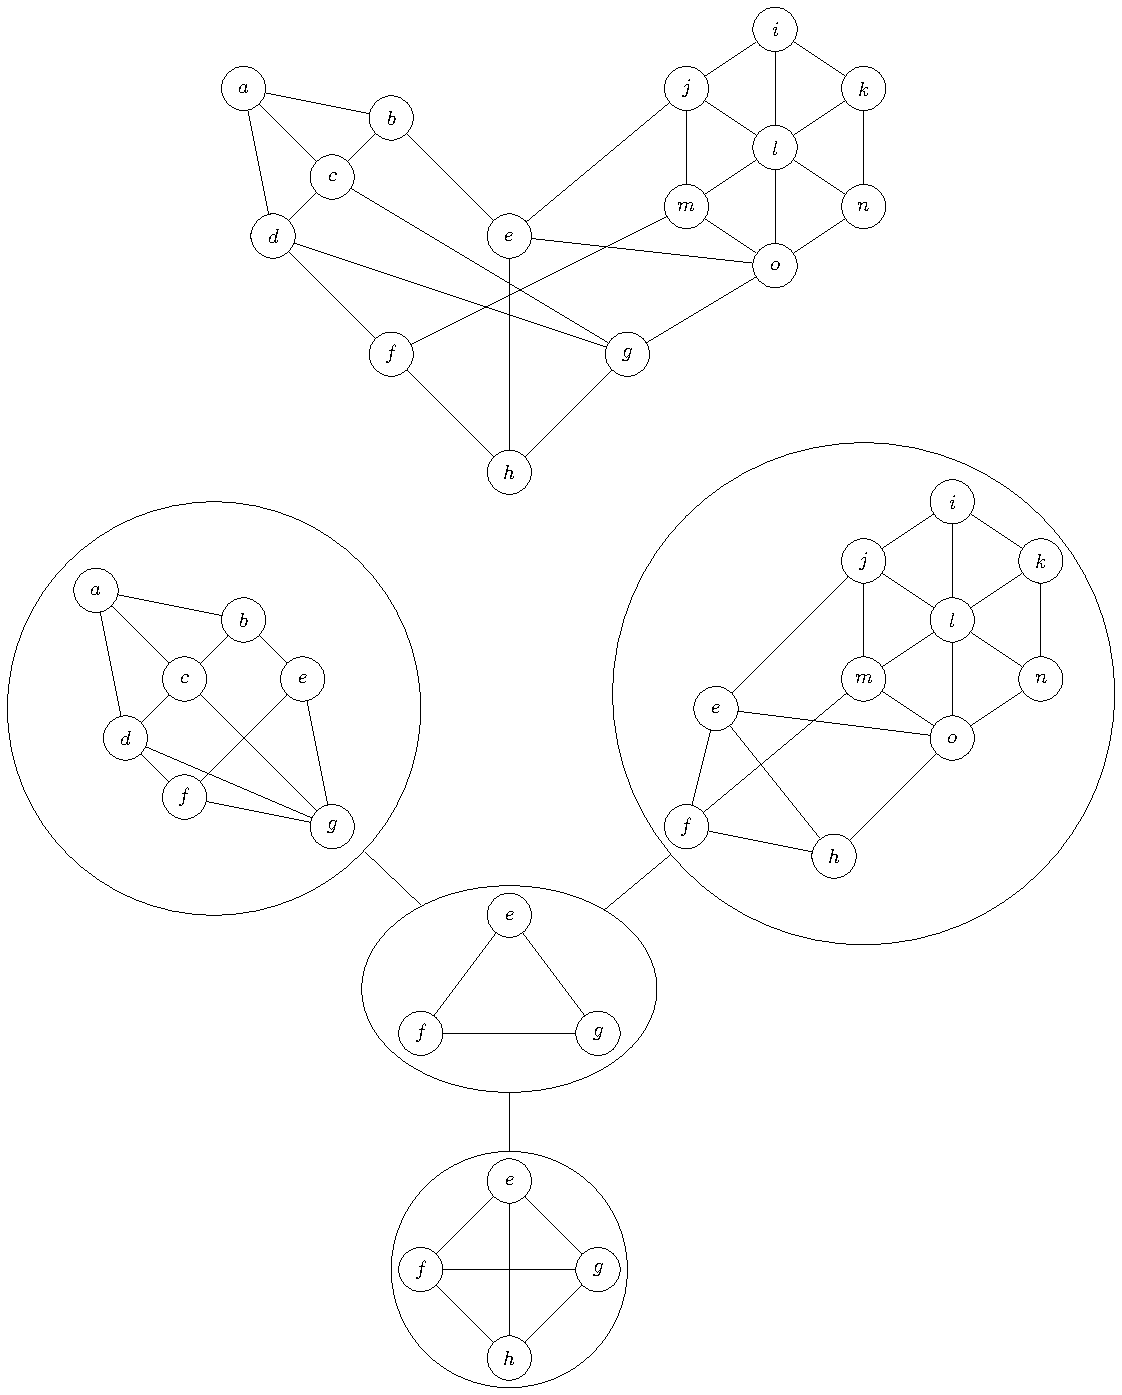
\includegraphics[width=\textwidth,height=\textheight,keepaspectratio]{bilder/33-Block-Tree.pdf}
  \caption{Ein $3$-zusammenhängender Graph mit dazugehörigem \dd-Block-Tree.
           Der Separator wird durch $\{e, f, g\}$ gebildet.
           Es ist zu sehen, dass der Eingabegraph nicht planar ist, da ein \kdd-Minor enthalten ist.
           Die Blockknoten enthalten jedoch alle planare Minoren des ursprünglichen Graphs.}
  \label{fig:33-Block-Tree}
\end{figure}


\subsection{Wagner-Struktur}
\begin{definition}\label{eq:WagnerStruktur}
  Sei $G$ ein Graph ohne \kf-Minor.
  Die \emph{Wagner-Struktur} von $G$ ist ein Wald von Bäumen, sodass für jede Zusammenhangskomponente $Z$ von $G$ genau ein Baum $T_Z$ existiert.
  Jeder $T_Z$ besteht aus einem $1$-Block-Tree $T_{(1)} = (V_{(1)}, E_{(1)})$ für $Z$, einem $2$-Block-Tree $T_{(2)} = (V_{(2)}, E_{(2)})$ für alle Graphknoten $v \in V_{(2)}$ und einem \dd-Block-Tree $T_{(3, 3)} = (V_{(3, 3)}, E_{(3, 3)})$ für alle Graphknoten $v \in V_{(2)}$\cite{ReL}.
\end{definition}

Die Wagner-Struktur von $G$ stellt eine Dekomposition dar, sodass alle Cliquenknoten $1$, $2$ und \dd-Separatoren von $G$ enthalten und die Graphknoten aller \dd-Block-Trees entweder planar oder isomorph zu $W$ sind.
Trifft das auf einen Graphknoten nicht zu, dann enthält $G$ einen \kf-Minor und die Wagner-Struktur ist ungültig.
Das Theorem von Wagner kann daraufhin wie folgt formuliert werden:

\begin{theorem}\label{eq:TheoremWagner}
  Ein Graph enthält genau dann keinen \kf-Minor, wenn für ihn eine Wagner-Struktur existiert\cite{Wag37}.
\end{theorem}

Als Beispiel ist dazu in \Abb \ref{fig:WagnerStruktur1} ein Graph $G$ zu sehen, der nicht planar ist, aber keinen \kf-Minor enthält.
In \Abb \ref{fig:WagnerStruktur2} sind die $3$-zusammenhängende Graphen $G_1$, $G_2$, $G_3$, $G_4$, $G_5$ und $G_6$ abgebildet, von denen ebenfalls keiner einen \kf-Minor enthält.
Außerdem ist $G_6$ nicht planar.
Einige Cliquen sind in beiden Abbildungen mit je einer Farbe hervorgehoben, sodass durch das Zusammenfügen gleichfarbiger Knoten ein Graph $G'$ erzeugt werden kann, der $G$ als Teilgraphen enthält.
In \Abb \ref{fig:WagnerStruktur3} ist die Wagner-Struktur zu $G$ skizziert.
Der $1$-Block-Tree wurde nicht eingezeichnet, da er aufgrund des $2$-Zusammenhangs von $G$ aus nur einem Graphknoten besteht.
Foglich existiert ein einzelner $2$-Block-Tree, der aus blauen Knoten und Kanten besteht.
Für jeden seiner Graphknoten existiert ein \dd-Block-Tree (rot).
Es kann beobachtet werden, dass die Cliquenknoten aller Block-Trees genau die farblich markierten Cliquen aus \Abb \ref{fig:WagnerStruktur2} enthalten und in $G$ Separatoren bilden.
Außerdem ist zu sehen, dass die Graphknoten aller \dd-Block-Trees entweder planar oder isomorph zu $W$ sind.
Daraus folgt, dass $G$ keinen \kf-Minor enthält.

\begin{figure}[H]
  \centering
  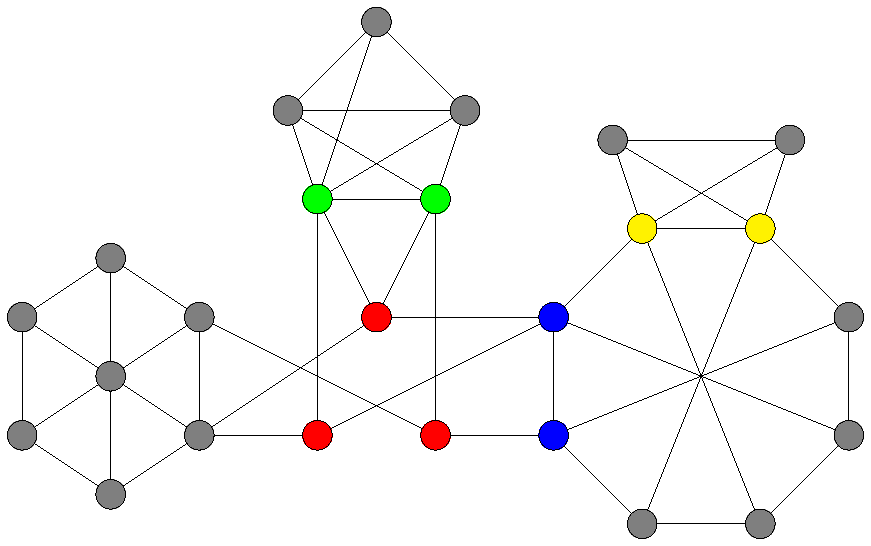
\includegraphics[width=\textwidth,height=\textheight,keepaspectratio]{bilder/WagnerTheorem1.pdf}
  \caption{Ein nicht-planarer Graph $G$, der keinen \kf-Minor enthält.}
  \label{fig:WagnerStruktur1}
\end{figure}

\begin{figure}[H]
  \centering
  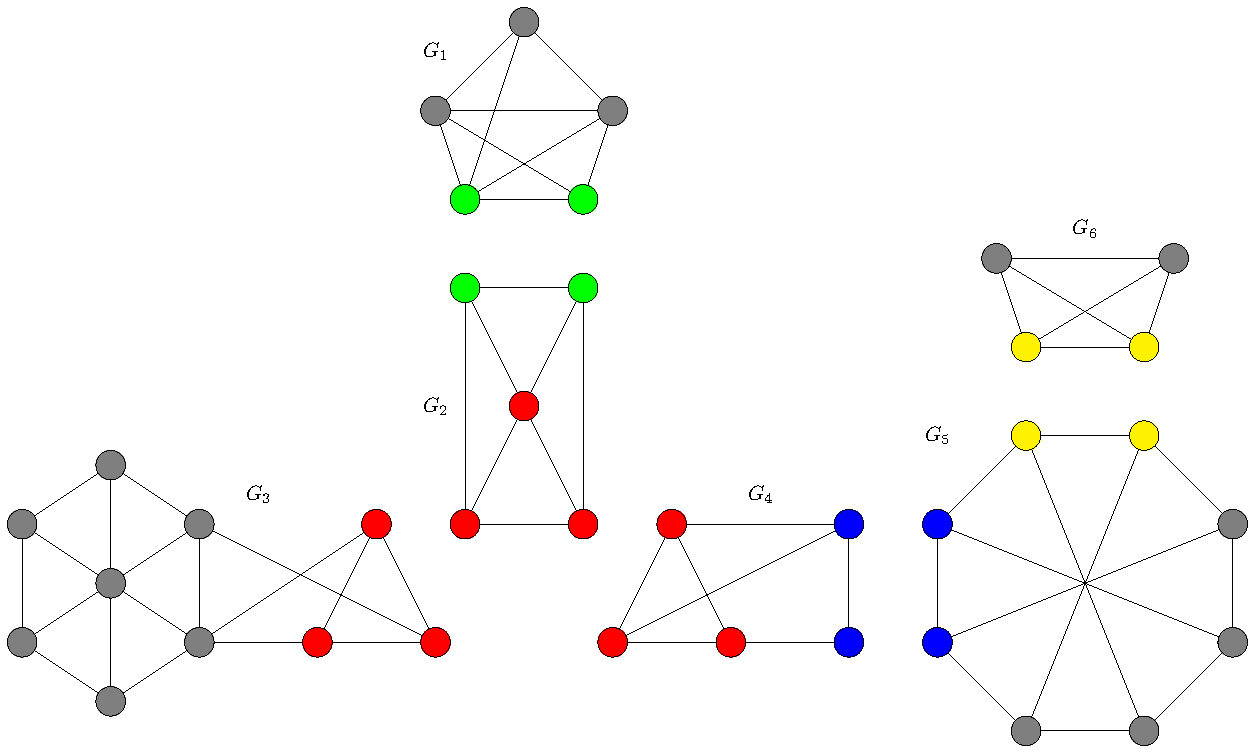
\includegraphics[width=\textwidth,height=\textheight,keepaspectratio]{bilder/WagnerTheorem2.pdf}
  \caption{Mehrere Graphen, die planar oder isomorph zu $W$ sind.}
  \label{fig:WagnerStruktur2}
\end{figure}

\begin{figure}[H]
  \centering
  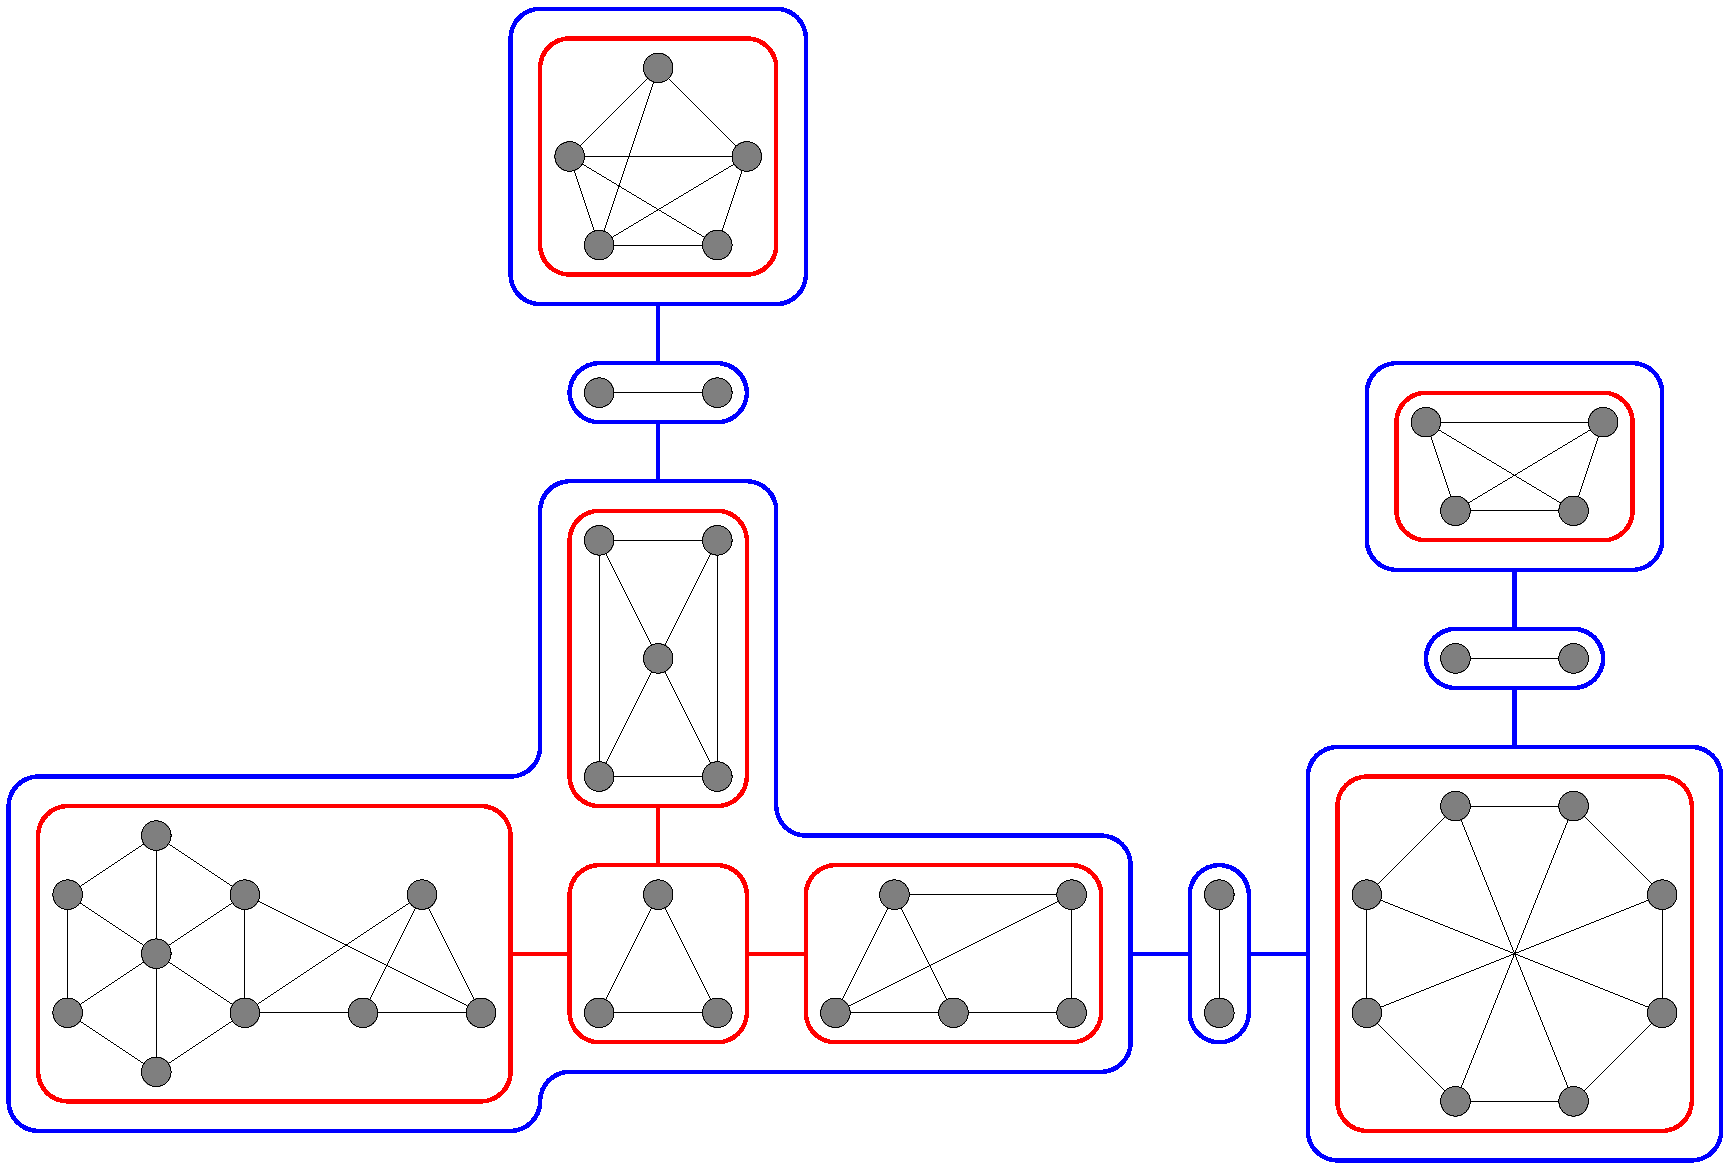
\includegraphics[width=\textwidth,height=\textheight,keepaspectratio]{bilder/WagnerTheorem3.pdf}
  \caption{Wagner-Struktur von $G$ aus \Abb \ref{fig:WagnerStruktur1}.
           Da $G$ bereits $2$-zusammenhängend ist, enthält der $1$-Block-Tree einen einzelnen Graphknoten für den kompletten Graphen und wurde nicht eingezeichnet.
           Die Knoten und Kanten des $2$-Block-Trees sind blau, die der \dd-Block-Trees rot hervorgehoben.}
  \label{fig:WagnerStruktur3}
\end{figure}

\section{Algorithmus von Kezdy und McGuinness als Wagner-Struktur}
Im Folgenden wird die durch Block-Trees definierte Wagner-Struktur mit dem Algorithmus von Kezdy und McGuinness verglichen und dieser so modifiziert, dass er sie erzeugen kann.
Anschließend werden augmentierte Komponenten für $1$- und $2$-Separatoren durch Block-Cut Trees und SPQR-Bäume erzeugt sowie ein zertifizierender Algorithmus beschrieben.

\subsection{Block-Trees}
\begin{beobachtung}
  Wird der Graph in augmentierte Komponenten aufgeteilt, sind diese isomorph zu mindestens einem Blockknoten der verschiedenen Block-Trees, wenn bis dahin alle Separatoren gleich gewählt wurden.
\end{beobachtung}
Im Algorithmus von Kezdy und McGuinness wird der Graph in augmentierte Komponenten aufgeteilt, wenn ein $(1, 2)$-, $(2, 2)$- oder \dd-Separator gefunden wird.
Sei $C$ ein solcher $(i, j)$-Separator, der einen zusammenhängenden Graphen $G$ in genau $j$ Zusammenhangskomponenten $Z_1, ..., Z_j$ aufteilt, wenn die $i$ Knoten von $C$ aus $G$ entfernt werden.

Angenommen, es gäbe eine augmentierte Komponenten $G_a$, zu der es im zugehörigen \dd-Block-Tree keinen Blockknoten $t$ mit assoziiertem Graphen $G_t$ gibt, sodass $G_a$ und $G_t$ isomorph sind.
Dann gibt es einen Separator $C_a$ in $G$, aus dem $G_a$ entstanden ist.
Da es kein $t$ mit einem zu $G_a$ isomorphen $G_t$ gibt, wurden keine Knoten im Block-Tree mit $C_a$ erzeugt, sodass es ebenfalls keinen Cliquenknoten mit $C_a$ gibt.
Dann wurde mindestens ein Separator $C_a'$ für den $1$-Block-Tree gewählt, wodurch die Knoten von $C_a$ so in Blockknoten enthalten sind, dass sie dort keinen Separator bilden, was der gleichen Wahl von Separatoren widerspricht.
Oder $C_a$ ist vollständig in einem Blockknoten enthalten und bildet dort einen Separator, was entweder dem $2$-Zusammenhang oder der Planarität \bzw Isomorphie zu $W$ des Blockknotens widerspricht.

Der Algorithmus von Kezdy und McGuinness erzeugt also zu Beginn alle Blockknoten eines $1$-Block-Trees.
Zusätzlich können die Knoten der gefundenen Separatoren gespeichert werden, um ebenfalls die Cliquenknoten zu erhalten, sodass der Algorithmus einen $1$-Block-Tree erzeugt.
Im zweiten Schritt werden die augmentierten Komponenten \bzw Blockknoten des $1$-Block-Tree in $3$-zusammenhängende augmentierte Komponenten \bzw einen $2$-Block-Tree überführt.
Analog zum vorherigen Fall gibt es für jede augmentierte Komponente, die aus einem Blockknoten des $1$-Block-Trees mit einem $(2, 2)$-Separator gebildet wird, einen isomorphen Blockknoten im $2$-Block-Tree, falls alle Separatoren gleich gewählt wurden.
Erneut können aus den Separatorknoten Cliquen gebildet und in zusätzlichen Knoten gespeichert werden, um als Ausgabe des zweiten Schrittes einen $2$-Block-Tree zu erzeugen.

Wird ein $1$-Block-Tree durch einen Block-Cut Tree aufgebaut, dann muss zusätzlich jedes adjazente Knotenpaar des Block-Cut Trees nach dem gemeinsamen Knoten durchsucht werden, der den $1$-Separator bildet.
Analog müssen für einen $2$-Block-Tree Knotenpaare des SPQR-Baumes, die aus zwei R-Knoten bestehen, nach den zwei gemeinsamen Knoten durchsucht werden, die ein $(2)$-Separator waren.
Neben den Knotenpaaren, die adjazent zueinander sind, müssen Cliquenknoten zusätzlich für solche gebildet werden, die durch einen Pfad miteinander verbunden sind, der ausschließlich aus S-, P- oder Q-Knoten besteht.
Um in der Praxis Laufzeit zu sparen, kann dieser Schritt auf den Fall verschoben werden, dass ein \kf-Minor gefunden wurde und die zugehörigen Pfade im Eingabegraph geprüft werden sollen.

Um die Blockknoten des $2$-Block-Trees in je einen \dd-Block-Tree zu verwandeln, müssen nicht nur entsprechende Separatoren gefunden und augmentierte Komponente gebildet, sondern auch garantiert werden, dass die Blockknoten der \dd-Block-Trees entweder planar oder isomorph zu $W$ sind und in keinem ein \kf-Minor enthalten ist.
Hier kann das Theorem \ref{eq:Theorem36} in Kombination mit dem zuvor angewendeten Planaritätstest genutzt werden, um die Struktur aufzubauen.
Sei dazu $G_t$ der Graph, der zu einem beliebigen Blockknoten $t$ im $2$-Block-Tree gehört.
$G_t$ muss $3$-zusammenhängend sein, da er als Graph vollständig in $t$ vorkommt.
Im Algorithmus von Kezdy und McGuinness wird $G_t$ nun im dritten Schritt durch einen Planaritätstest überprüft.
Wird ein \kf-Minor gefunden, ist die Wagner-Struktur ungültig und der Algorithmus terminiert.
Andernfalls kann $G_t$ planar sein -- dann wird im \dd-Block-Tree ein einzelner Blockknoten angelegt, der $G_t$ enthält und als planar markiert ist.
Letztlich kann der Planaritätstest ein \kdd-Subdivision $S$ finden, sodass die Voraussetzungen für Theorem \ref{eq:Theorem36} gegeben sind.
Im ersten Fall von Theorem \ref{eq:Theorem36} enthält $G_t$ jedoch einen \kf-Minor, da keine Knoten von $S$ einen \dd-Separator bilden -- der Beweis dazu findet sich in Lemma \ref{eq:Lemma35}.
Damit wäre die Wagner-Struktur erneut ungültig.
Im zweiten Fall ist $G_t$ isomorph zu $W$.
Analog zum planaren Fall wird ein neuer Blockknoten im \dd-Block-Tree angelegt, der $G_t$ enthält und entsprechend gekennzeichnet ist.
Der dritte und vierte Fall treten ein, falls drei Knoten aus $S$ einen \dd-Separator bilden.
Kezdy und McGuinness erzeugen hier augmentierte Komponenten, die als Blockknoten des \dd-Block-Trees genutzt werden können.
Zusätzlich müssen die drei Knoten des Separators als neuer Cliquenknoten eingefügt und mit den entstandenen Blockknoten verbunden werden.
Der Algorithmus wird rekursiv auf jeden der Blockknoten angewendet, bis alle zugehörigen Teilgraphen planar oder isomorph zu $W$ sind \bzw ein \kf-Minor gefunden wurde.
Somit ist das Ergebnis des modifierten Algorithmus entweder eine Wagner-Struktur, die aus einem Wald von $1$-Block-Trees mit Blockknoten, die aus $2$-Block-Trees mit Blockknoten aus \dd-Block-Trees bestehen und die die planaren Minoren und Kopien von $W$ im Eingabegraph zeigen.
Oder es wird ein \kf-Minor als Teilgraph des Eingabegraphen gefunden, sodass die Wagner-Struktur ungültig ist, die Frage, ob ein \kf-Minor enthalten ist, jedoch in beiden Fällen eindeutig beantwortet werden kann.

\subsection{Zertifierender Algorithmus}
Das Ziel ist, einen \kf-Minor zu finden oder ein Zertifikat zu liefern, dass keiner enthalten ist.
Dafür sind besonders folgende Strukturen in einem Graphen relevant: Planare Teilgraphen, $W$-Subdivisions, \kf-Minoren und \dd-Separtoren -- andere Separatoren werden lediglich benötigt, um den $3$-Zusammenhang zu garantieren.
Beispielsweise sind zwei planare Teilgraphen, die durch einen $2$-Separator verbunden sind, ebenfalls planar.
Das Zertifikat für einen Graphen $G$ besteht also entweder aus einem gefundenen \kf-Minor in Form von fünf disjunkten Knotenmengen, die jeweils einen der fünf Knoten des \kf formen -- dann ist zu prüfen, ob dadurch im ursprünglichen Graph ebenfalls einer geformt wird.
Einerseits muss dazu jede Knotenmenge einen zusammenhängenden Teilgraphen in $G$ formen.
Andererseits sind genau diese fünf Teilgraphen paarweise durch Pfade in $G$ verbunden, die beispielsweise durch eine Tiefensuche gefunden werden können.
Oder es wird eine Wagner-Struktur erzeugt, es kann jeder Knoten der Struktur wie folgt geprüft werden:
\begin{enumerate}
  \item \textbf{Planar}: Sei $G'$ der Teilgraph von $G$, der alle Knoten des planaren Minoren enthält.
        Dann ist $G'$ ebenfalls planar, was \zB durch einen Planaritätstest geprüft werden kann.
  \item \textbf{$W$}: Analog zum Test eines \kf-Minor können acht Knotenmengen die $W$-Subdivision darstellen.
        Der für den Algorithmus von Kezdy und McGuinness implementierte Isomorphietest kann wiederverwendet werden. % TODO: Isomorphietest in Implementierung beschreiben
  \item \textbf{\dd-Separator}: Jeder gefundene Separator bildet auch im ursprünglichen Graphen einen Separator.
        Sei $a$ die Anzahl der Zusammenhangskomponenten von $G$.
        Dann kann der \dd-Separator aus $G$ entfernt werden.
        Sei $b$ die neue Anzahl der Zusammenhangskomponenten.
        Dann muss $b - a \geq 2$ gelten.
\end{enumerate}
